\documentclass[12pt, oneside]{article}
\usepackage[letterpaper, margin=1in, headsep=0.5in]{geometry}
\usepackage[english]{babel}
\usepackage[utf8]{inputenc}
\usepackage{amsmath}
\usepackage{amsfonts}
\usepackage{amssymb}
\usepackage{tikz}
\usetikzlibrary{quotes, angles}
\usepackage{graphicx}
%\usepackage{pgfplots}
%\pgfplotsset{width=10cm,compat=1.9}
%\usepgfplotslibrary{statistics}
%\usepackage{pgfplotstable}
%\usepackage{tkz-fct}
%\usepackage{venndiagram}

\usepackage{fancyhdr}
\pagestyle{fancy}
\fancyhf{}
\rhead{\thepage \\Name: \hspace{1.5in}.\\}
\lhead{BECA / Dr. Huson / Geometry 10th Grade\\* Unit 2: Introduction to Proof\\5 November 2018}

\renewcommand{\headrulewidth}{0pt}

\begin{document}
\subsubsection*{Do Now: Formulating geometric situations}
  \vspace{0.5cm}
  Use the postulates and theorems you have learned. You may abbreviate them as follows: ``def. of bisector," ``$\perp$ rays meet at $90^\circ$," ``complementary $\angle$s add to 90," ``linear pairs add to 180," ``vertical $\angle$s are $\cong$,"

  \begin{enumerate}

\subsubsection*{Circle the appropriate equation and state the justification}

  \item Given complementary angles, $\angle A$, $\angle B$.\\[0.5cm]
  $\angle A \cong \angle B$ \hspace{1cm} $m \angle A + m \angle B=90^\circ$ \hspace{0.5cm} \rule{5cm}{0.15mm} \vspace{0.25cm}

  \item $\angle RPS \cong \angle SPU$ \hspace{0.25cm} $m \angle RPS + m \angle SPU = 180^\circ$ \hspace{0.25cm} \rule{6cm}{0.15mm}  \vspace{0.25cm}
      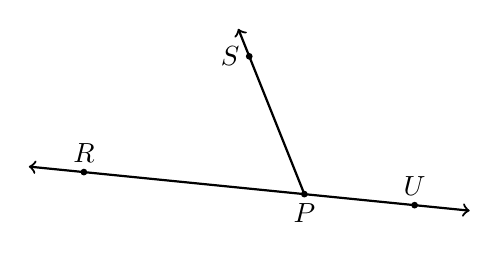
\begin{tikzpicture}[scale=0.7]
        \draw [<->, thick] (-5,.5)--(3,-.3);
        \draw [->, thick] (0,0)--(-1.2,3);
        \draw [fill] (-1,2.5) circle [radius=0.05] node[left ]{$S$};
        \draw [fill] (0,0) circle [radius=0.05] node[below]{$P$};
        \draw [fill] (2,-0.2) circle [radius=0.05] node[above]{$U$};
        \draw [fill] (-4,0.4) circle [radius=0.05] node[above]{$R$};
      \end{tikzpicture}

  \item Given $m \angle 1 = 4x+6$, $m \angle 2 = 6x-32$. Find $m \angle 1$.
      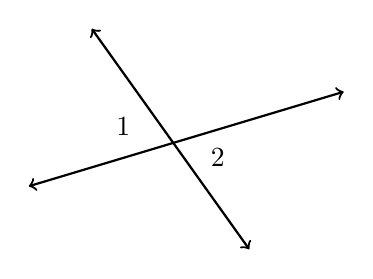
\begin{tikzpicture}[scale=.4]
        \draw [<->, thick] (0,-1.5)--(10,1.5);
        \draw [<->, thick] (2,3.5)--(7,-3.5);
        \node at (3,.4){1};
        \node at (6,-.6){2};
      \end{tikzpicture}\\[0.5cm]
      $\angle 1 \cong \angle 2$ \hspace{1cm} $m\angle 1 + m\angle 2 =  180$ \hspace{0.5cm} \rule{6cm}{0.15mm}

  \item Given $m\angle R=50$, $m\angle U =65$, and $m\angle UST=115$. Find $m\angle RSU$.
  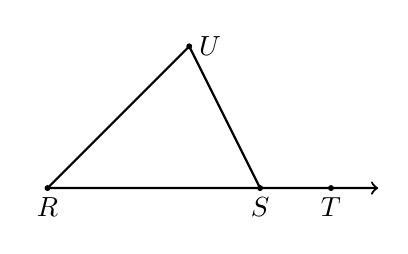
\begin{tikzpicture}[scale=0.6]
    %\draw [->, thick] (0,0)--(5,5);
    \draw [<-, thick] (7,0)--(0,0)--(3,3)--(4.5,0);
    \draw [fill] (0,0) circle [radius=0.05] node[below]{$R$};
    \draw [fill] (4.5,0) circle [radius=0.05] node[below]{$S$};
    \draw [fill] (3,3) circle [radius=0.05] node[right]{$U$};
    \draw [fill] (6,0) circle [radius=0.05] node[below]{$T$};
  \end{tikzpicture}\\[0.5cm]
  $\angle UST \cong \angle RSU$ \hspace{0.5cm} $m\angle UST + m\angle RSU =  180$ \hspace{0.5cm} \rule{6cm}{0.15mm} \vspace{0.5cm}

  \item Given $\overrightarrow{BA} \perp \overrightarrow{BC}$, $m \angle ABD = 2x-5$, and $m \angle DBC = x-10$.
    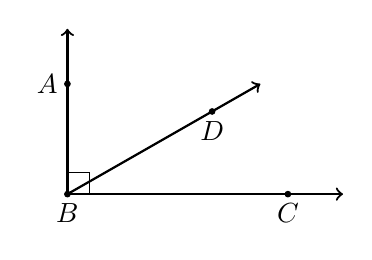
\begin{tikzpicture}[scale=0.7]
      \draw [<->, thick] (0,3)--(0,0)--(5,0);
      \draw [->, thick] (0,0)--(3.5, 2);
      \draw [-, thin] (0, 0.4)--(0.4, 0.4)--(0.4, 0);
      \draw [fill] (0,0) circle [radius=0.05] node[below]{$B$};
      \draw [fill] (0,2) circle [radius=0.05] node[left]{$A$};
      \draw [fill] (4,0) circle [radius=0.05] node[below]{$C$};
      \draw [fill] (2.625, 1.5) circle [radius=0.05] node[below]{$D$};
    \end{tikzpicture}\\[0.5cm]
    $\angle ABD \cong \angle DBC$ \hspace{0.5cm} $m\angle ABD + m\angle DBC =  90$ \hspace{0.5cm} \rule{6cm}{0.15mm}

\newpage

  \item Prove the quadrilateral $BECA$ with $B(1, 3)$, $E(3, 2)$, $C(5,6)$, and $A(3, 7)$ is a rectangle, using the theorem "If a quadrilateral's diagonals are congruent, then it is a rectangle."
  \begin{enumerate}
    \item Plot and label the points on the graph. Draw $BECA$.
    \item Draw the diagonals, $\overline{BC}$ and $\overline{EA}$.
    \item Find the length of $EA$, showing the subtraction of the $y$ values.
    \item Find $BC$ using the distance formula.
  \end{enumerate}
  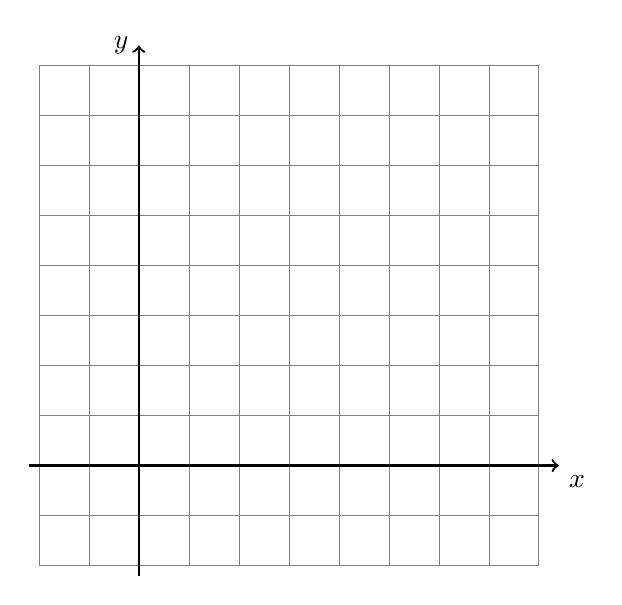
\begin{tikzpicture}[scale=.635]
    \draw [help lines] (-2,-2) grid (8,8);
    \draw [thick, ->] (-2.2,0) -- (8.4,0) node [below right] {$x$};
    \draw [thick, ->] (0,-2.2)--(0,8.4) node [left] {$y$};
  \end{tikzpicture}

  \item Given the circle $C$ with circumference $6\pi$.
  \begin{enumerate}
    \item Write down the formula for the circumference of a circle. \vspace{1.5cm}
    \item Solve for the radius yielding a circumference of $6\pi$. \vspace{2cm}
    \item Find the area of the circle.
  \end{enumerate}
  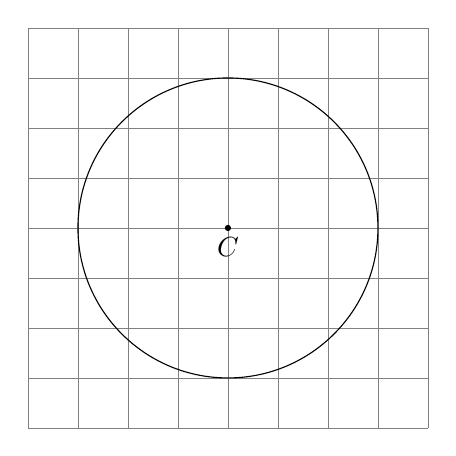
\begin{tikzpicture}[scale=.635]
    \draw [help lines] (-4,-4) grid (4,4);
    %\draw [thick, ->] (-2.2,0) -- (10.4,0) node [below right] {$x$};
    %\draw [thick, ->] (0,-2.2)--(0,10.4) node [left] {$y$};
    \draw (0,0) circle [radius=3] node[below]{$C$};
    \draw [fill] (0,0) circle [radius=0.05];
  \end{tikzpicture}

  \end{enumerate}

\end{document}
